\documentclass[conference]{IEEEtran}
\IEEEoverridecommandlockouts
% The preceding line is only needed to identify funding in the first footnote. If that is unneeded, please comment it out.
\usepackage{cite}
\usepackage{amsmath,amssymb,amsfonts}
\usepackage{algorithmic}
\usepackage{graphicx}
\usepackage{textcomp}
\usepackage{placeins}
\usepackage{adjustbox}
\usepackage{booktabs}
\usepackage{xcolor}
\usepackage[normalem]{ulem}
\usepackage{caption}
\usepackage{subcaption}
\useunder{\uline}{\ul}{}
\def\BibTeX{{\rm B\kern-.05em{\sc i\kern-.025em b}\kern-.08em
    T\kern-.1667em\lower.7ex\hbox{E}\kern-.125emX}}

% !TeX spellcheck = en_GB 

\begin{document}

\title{Decision Trees for exploratory analysis of Legendary-Pokémon and their predictors}

\author{\IEEEauthorblockN{Pascal Quindeau}
\IEEEauthorblockA{\textit{University of Niederrhein}\\
Krefeld, Germany \\
quindeau.pascal@gmail.com}
\and
\IEEEauthorblockN{Name Surname}
\IEEEauthorblockA{\textit{name of organization (of Aff.)}\\
City, Country \\
email address}

}

\maketitle

\begin{abstract}
In this paper, we first scrape relevant Pokémon data from two distinct websites and further use it to explore different distributions among Pokémon labelled as either \textit{Non-Legendary}, \textit{Sub-Legendary}, \textit{Mythical} and \textit{Legendary}. We identify several possible predictors that might give a Pokémon its \textit{Legendary} status, such as its \textit{Stats}, its first and second \textit{Type}, its \textit{Growth Rate} and even its \textit{Height}. Finally, we use a decision tree model to get more insight into how these multiple predictors function together to distinct between \textit{Legendary} and \textit{Non-Legendary} Pokémon. Our decision tree models achieves an \textit{accuracy score} of $0.964$ which is roughly $6\%$ better than the baseline model.
\end{abstract}

\begin{IEEEkeywords}
Data Science, Decision Tree, Pokémon, Exploratory Analysis
\end{IEEEkeywords}

\section{Introduction}
In recent years, Data Science has emerged as an important discipline for business companies, individuals and even society \cite{aalst16}. Van der Aalst refers to it as an ''amalgamation of classical disciplines like statistics, data mining, data bases and distributed systems''. In this paper, we are mostly interested in data mining and statistics. For the sole data mining purpose, Fayadd et al. discuss the need of Data Mining as a discipline of knowledge discovery in databases (short KDD) in \cite{fayyad96} as data in its raw format is mostly abstract. A statistician, data scientist or analyst has first to transform the data into some more compact and useful form. Here, a data science project usually follows a given pattern:
\begin{enumerate}
	\item Selection: Select the needed data from a larger data storage. This could be a file, a database or even the web. 
	\item Preprocessing: Transform the data, for example from unstructured to structured or introduce new features as a combination of other features.
	\item Transformation: Transform the data into a valid format that is helpful for the analysis task.
	\item Data Mining: Use specific Data Mining tools, like exploratory models, descriptive statistics and more.
	\item Interpretation/ Evaluation: Conclude your findings and add them as new or confirmed knowledge.
\end{enumerate}
For this paper, we decided to mirror the aforementioned approach. Here, we use Data Mining and Data Science interchangeable as we are mostly interested in extracting new knowledge from our data and not how to distribute it or store it efficiently in a database. Our data domain will be Nintendo's most liked Pokémon-Franchise\footnote{See https://www.pokemon.com/de/ for more information about Pokémon.}. Pokémon is a well known and well understood phenomenon among young people and even adults. The data is publicly available on several websites and can be easily scraped via Tools like scrapy\footnote{https://scrapy.org/}.\\
This paper will be structured as follows: First, we talk about the data collecting and preprocessing step. For this, we scrape two websites, one for the general Pokémon data and one for the target variable. Next, we provide some exploratory inside into the data itself and form multiple hypothesis based on distribution plots and pivot charts. At last, we train a decision tree model on a subsample of the overall available data and report its accuracy as well as the exploratory insight that a decision tree provides.
\section{Data preparation}
\subsection{Scraping the data}
\label{subsec:scraping}
The data is collected from two different website. The general Pokémon Database\footnote{https://pokemondb.net/pokedex/} provides a list of all Pokémon sorted by their national Dex number. This is further known as a \textit{National Pokédex}. A \textit{Dex} number is a unique identifier for each Pokémon. Currently, it is made up of a three digit integer preceded by a \#. Due to its uniqueness it can be used as a primary key if stored in a database. The list can be easily scraped using the Python framework scrapy. For each Pokémon, scrapy will follow the response to the Pokémon's actual web page, that we further use to extract meaningful data.
% Please add the following required packages to your document preamble:
% \usepackage[normalem]{ulem}
% \useunder{\uline}{\ul}{}
\begin{table*}[t]
	\centering
	\caption{Overview of extracted data from the Pokémon Database.}
	\begin{tabular}{ll} \hline
		\textbf{Feature}      & \textbf{Description}                                                                                                                                                                                                                         \\ \hline
		Dex Number            & A Pokémon's unique identifier.                                                                                                                                                                                                               \\
		Name                  & A Pokémon's name.                                                                                                                                                                                                                            \\
		First and second Type & A Pokémon's typing. Categorical value.                                                                                                                                                                                                       \\
		Height                & A Pokémon's height. Numerical value.                                                                                                                                                                                                         \\
		Weight                & A Pokémon's weight. Numerical value.                                                                                                                                                                                                         \\
		Stats                 & \begin{tabular}[l]{@{}l@{}}A Pokémon's statistics. Including Attack, \\ Defense, Special Attack, Special Defense, \\ Speed, Health Points and Total, whereas Total\\ is the sum of all stats. Numerical values.\end{tabular}                 \\
		Catch Rate            & \begin{tabular}[c]{@{}l@{}}The rate of successfully catching a Pokémon. It \\ reaches from 0 (low) to 255 (high). Numerical value.\end{tabular}                                                                                                \\
		Growth Rate           & \begin{tabular}[c]{@{}l@{}}The rate determining how much experience a Pokémon\\ needs to reach a certain level. Can be one of the following:\\ Erratic, Fast, Medium Fast, Medium Slow, Slow, Fluctuating.\\ Categorical value.\end{tabular} \\
		Male                  & Indicating whether a Pokémon can be male. Binary value.                                                                                                                                                                                      \\
		Female                & Indicating whether a Pokémon can be female. Binary value.                                                                                                                                                                                    \\
		Male Rate             & The probability of a Pokémon being male. Numerical value.                                                                                                                                                                                    \\
		Female Rate           & The probability of a Pokémon being female. Numerical value.                                                                                                                                                                                  \\
		Gen                   & The Gen in which a Pokémon first was introduced.  \\ \hline                                                                                                                                                                                          
	\end{tabular}
\label{tab:overview}
\end{table*}
Table \ref{tab:overview} gives an overview of the scraped features. Note that some of these might be missing for several Pokémon. A Pokémon might not have a second \textit{Type} as it is single typed. Some Pokémon like "Zarude" were only introduced recently and are not available to the game yet. Thus, data is missing. Another problem with using Pokémon Database lies in the way, the website stores special evolutions like \textit{Mega Evolutions}. These are listed under the same name and \textit{Dex} entry and cannot be extracted for a given Pokémon without overwriting it's first occurrence in a database. Thus, we decided to not include these evolutions in our database.\\
To extract label information, such as \textit{Non-Legendary}, \textit{Legendary}, \textit{Sub-Legendary} and \textit{Mythical}, we use Serebii.net\footnote{https://www.serebii.net/pokemon/legendary.shtml}.
\begin{table}[b]
	\centering
	\caption{Distribution of Pokémon among labels.}
	\label{tab:labels}
	\begin{tabular}{lr} \hline
		\textbf{Label} & \textbf{Count/Frequency} \\ \hline
		Non-Legendary  & 806/0.902                \\
		Sub-Legendary  & 42/0.047                 \\
		Mythical       & 23/0.026                 \\
		Legendary      & 22/0.025                 \\ \hline
	\end{tabular}
\end{table}
This site lists all Pokémon categorized by the aforementioned labels. We then use a Pokémon's \textit{Dex} number to combine both datasets. In the end, we extract $893$ Pokémon. The overall distribution of labels among different Pokémon can be seen in table \ref{tab:labels}. It shows a high skew towards \textit{Non-Legendary} Pokémon. Around $90\%$ of Pokémon are \textit{Non-Legendary}. We have to keep this information in mind, when training our decision tree classifier later. 
\section{Exploratory analysis}
In this section, we explore several possibilities for predictors that could help to distinct \textit{Legendary} from \textit{Non-Legendary} Pokémon. We do this by looking at different kinds of plots and descriptive values among the different labels. Based on the finding, we can then formulate specific hypothesises. This is not common in statistics, where scientists usually first formulate a hypothesis and try to proof it by analysing the given data. In this paper, however, we just want to give a short overview about basic exploratory techniques.
\subsection{Stats Distribution}
First, we want to investigate a Pokémon's stats (short for statistics). Here, we use a very versatile seaborn\footnote{https://seaborn.pydata.org/} function, called \textit{pairplot}. A pairplot shows the interaction between a set of variables on a matrix grid. Each cell corresponds two one combination. Combinations of different variables show scatter plots, whereas combinations of same variables show a distribution in form of a histogram or kernel density estimation (kde).
\begin{figure*}[t]
	\centering
	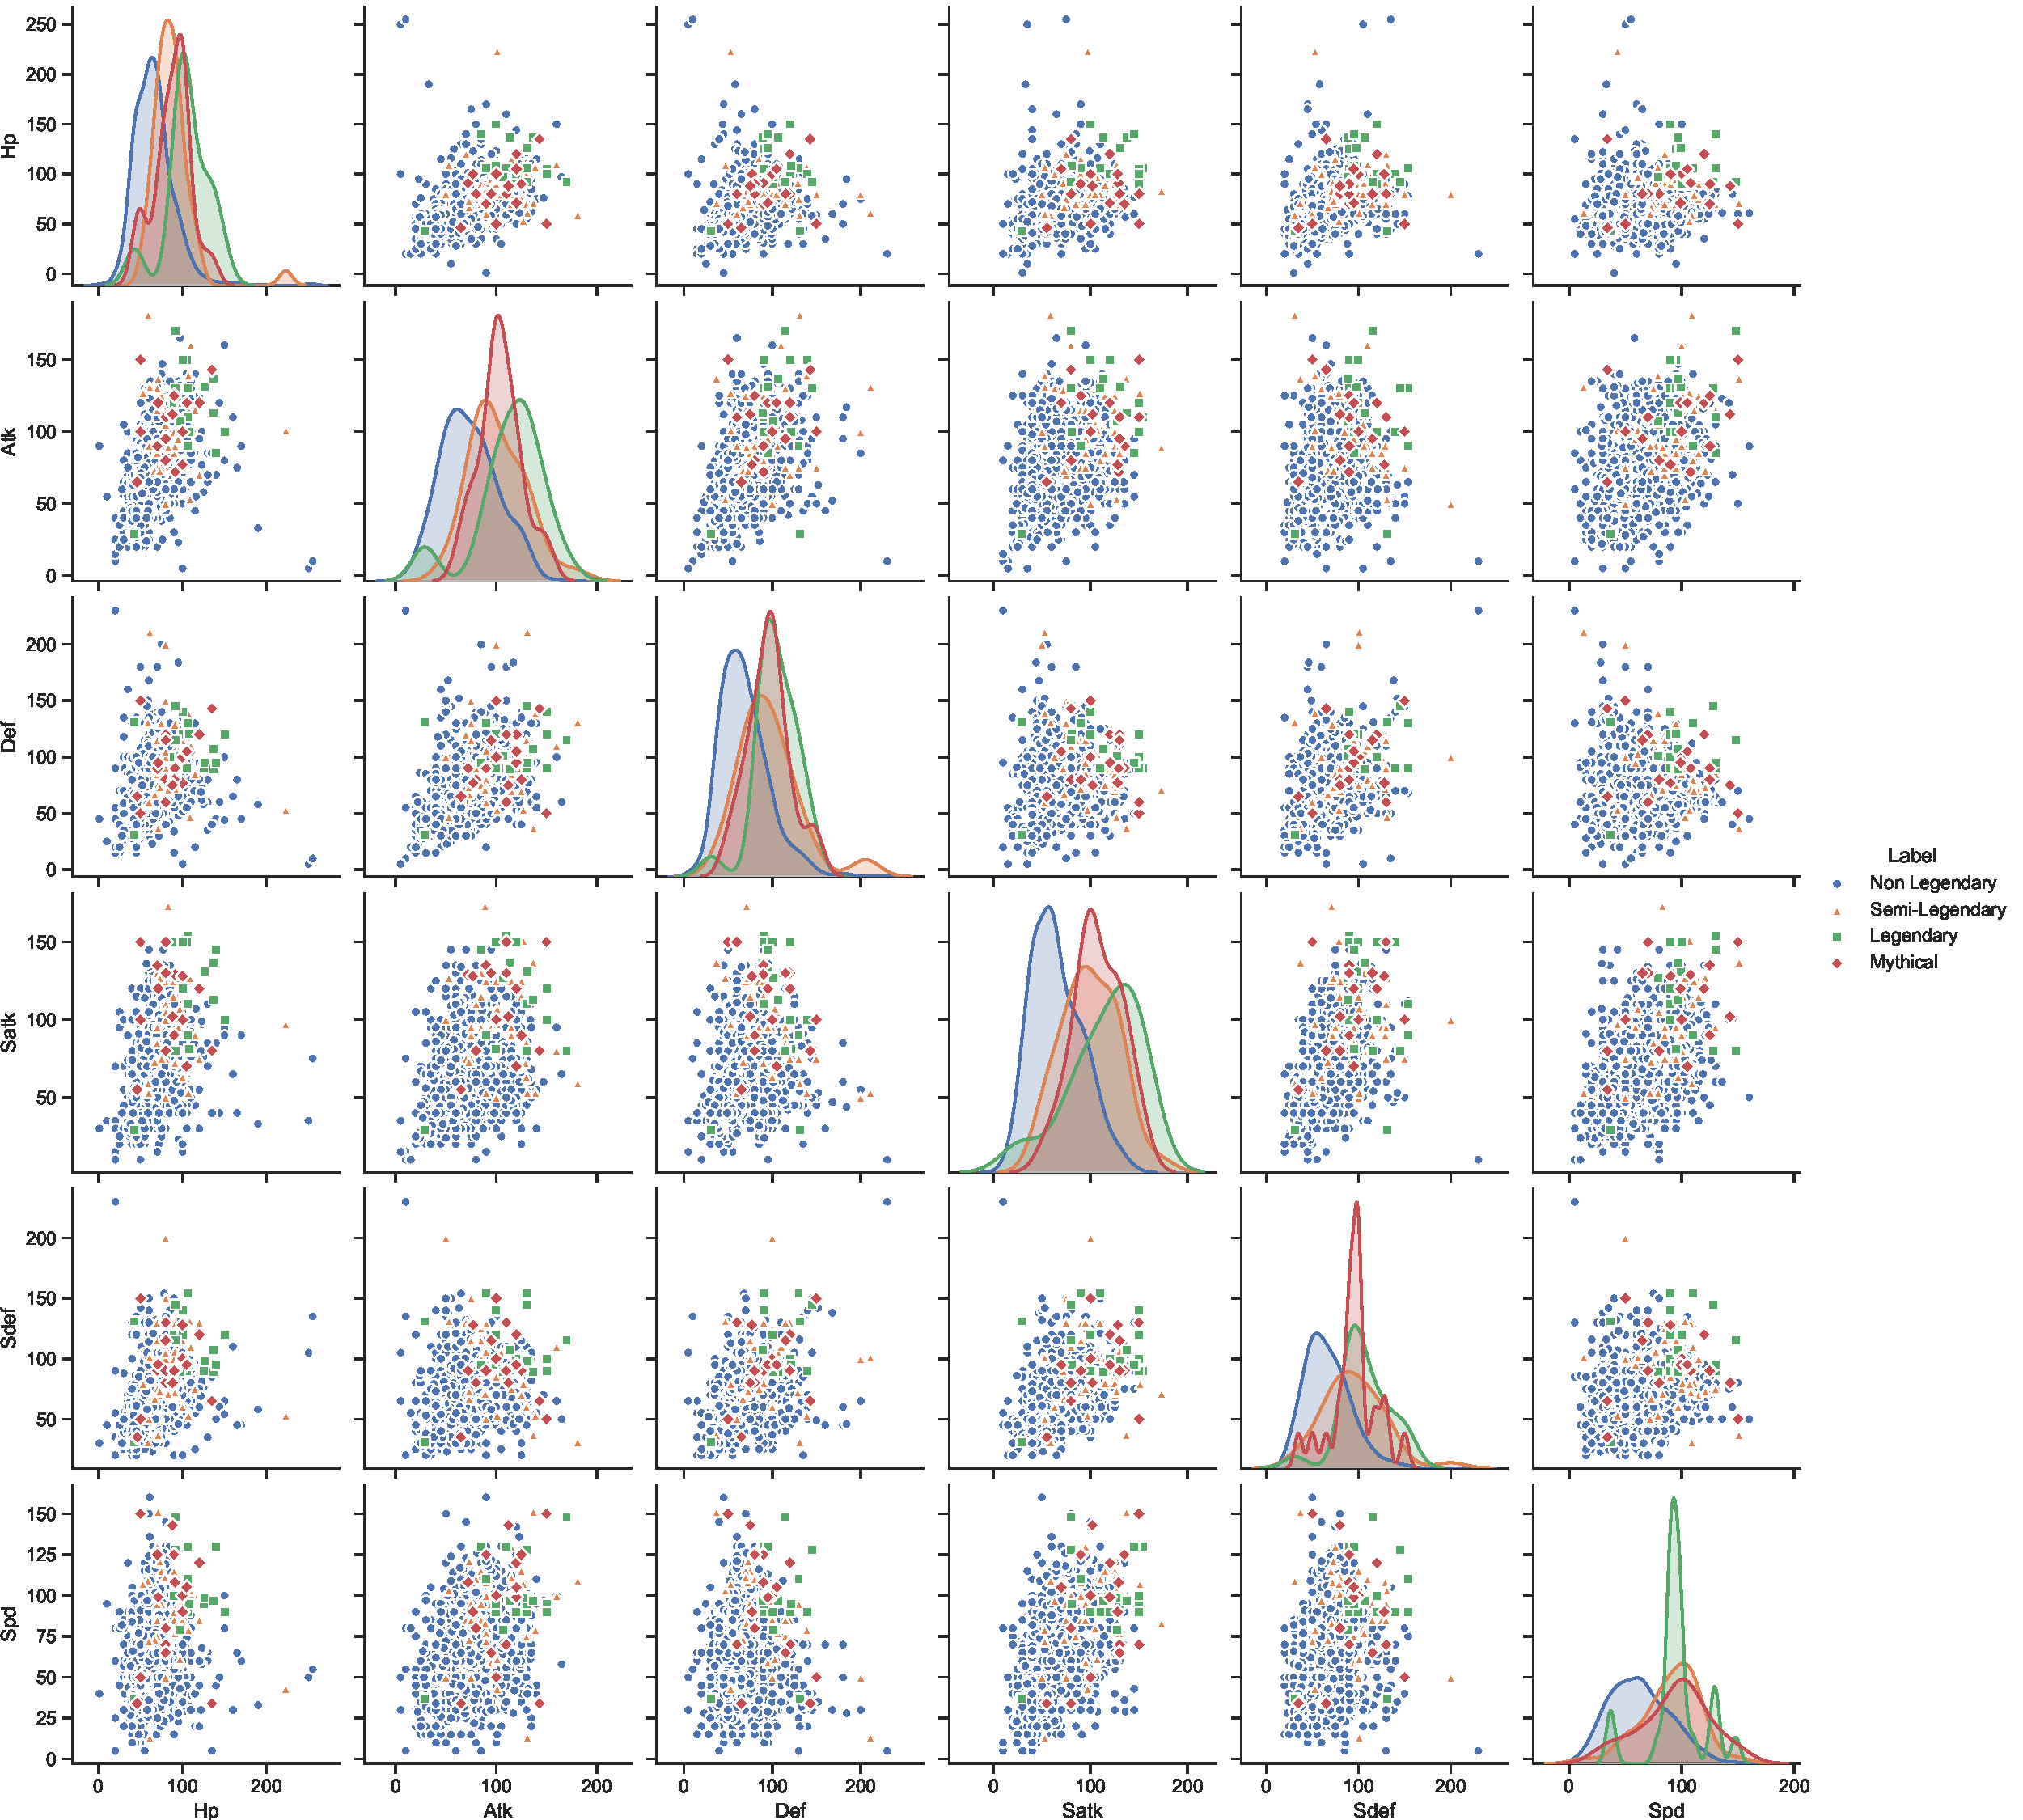
\includegraphics[width=\linewidth]{../../figures/pairplot_hue_coded.pdf}
	\caption{Pairplot of Health Points (HP), Attack (Atk), Defense (Def), Special Attack (Satk), Special Defense (Sdef) and Speed (Spd). The labels are colour and shape coded.}
	\label{fig:pairplot}
\end{figure*}
Figure \ref{fig:pairplot} shows the aforementioned pairplot for all Pokémon and their stats. It is notable, that most \textit{Non-Legendary} Pokémon lie in the bottom left of each given plot. Moreover, there seems to be a correlation between Hp and Atk as well as Spd and Satk. Indeed the correlation happens to be $0.46$ and $0.42$, respectively. The different distributions among the stats are most prominent in the offensive stats (Atk, Satk and Spd). Especially \textit{Legendary} Pokémon tend to differ strongly from \textit{Non-Legendary} Pokémon. This effect is more subtle for \textit{Sub-Legendary} Pokémon. This leads to our first hypothesis: 
\begin{enumerate}
	\item \textit{Non-Legendary} Pokémon tend to have lower stats, than other Pokémon.
\end{enumerate}
It might be, that the difference among stats is only due to non evolved Pokémon in the \textit{Non-Legendary} group. Usually, \textit{Legendary}, \textit{Mythical} and \textit{Sub-Legendary} already have reached their final form, whereas \textit{Non-Legendary} Pokémon may go through two or three stage in their life. That is, why one might observe a bimodal distribution among \textit{Non-Legendary} Pokémon. This, however, is not the case.
\subsection{Height and weight distribution}
Next, we report our findings on a Pokémon's height and weight. Especially \textit{Legendary} Pokémon tend to be large and ominous looking beasts. Pokémon like Kyogre\footnote{https://www.pokewiki.de/Kyogre} and Groudon\footnote{https://www.pokewiki.de/Groudon} come to mind. Kyogre weights 352.0 Kg with a height of 4.5m where Groudon is a real heavy weight with 950 Kg and 3.5m. The dataset contains two Pokémon with a maximal weight of 999.9 Kg. These are Cosmoem and Celesteela. The largest Pokémon, however, is the new \textit{Legendary} Pokémon called Eternatus with a height of 20.0m. 
\begin{figure}[h]
	\centering
	\begin{subfigure}{0.4\textwidth}
		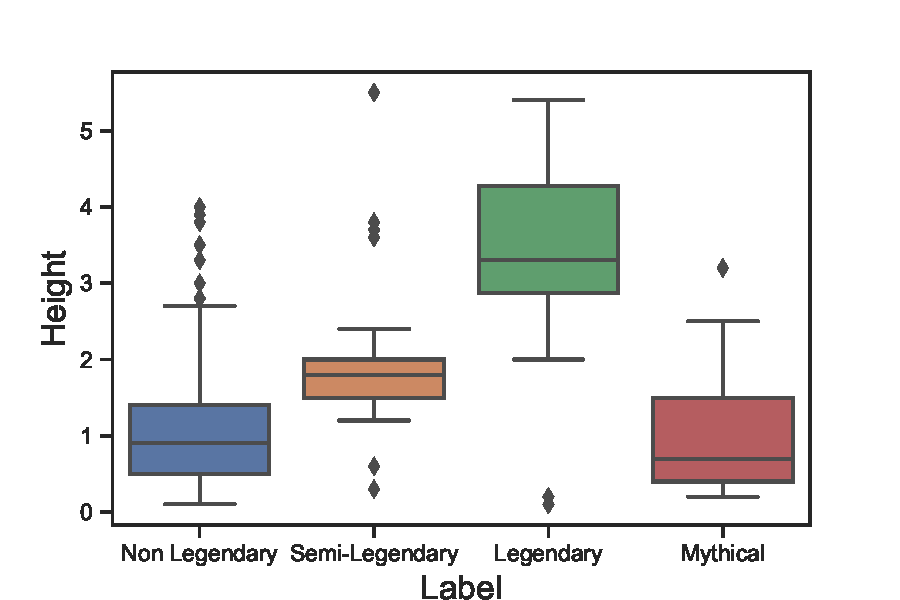
\includegraphics[width=\textwidth]{../../figures/boxplot_height.pdf}
		\caption{Height}
	\end{subfigure}
	\begin{subfigure}{0.4\textwidth}
	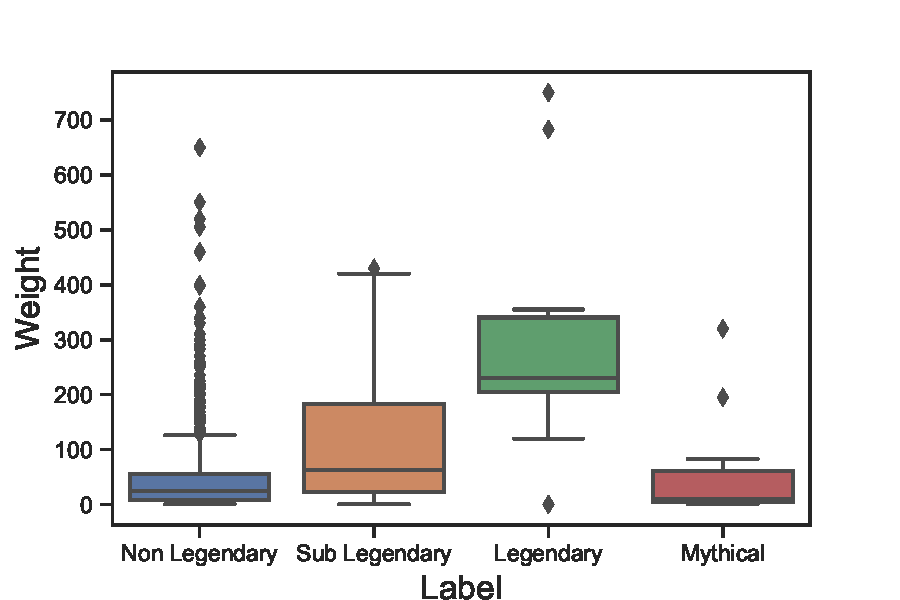
\includegraphics[width=\textwidth]{../../figures/boxplot_weight.pdf}
	\caption{Weight}
\end{subfigure}
\caption{Boxplot of the height and weight distribution among the different Pokémon classes.}
\label{fig:boxplot}
\end{figure}\\
Figure \ref{fig:boxplot} shows the height and weight distribution as two boxplots. At first glance, we observe the large difference in height between \textit{Legendary} and other Pokémon. This shows, that \textit{Legendary} Pokémon indeed are larger than other Pokémon. This effect is not as pronounced on \textit{Sub-Legendary} Pokémon, where $75\%$ lie between 1.5 to 2.0 metres. In section \ref{sec:type}, we talk about the influence on a Pokémon's first and second Type. A lot of \textit{Legendary} Pokémon tend to be either Dragon or Psychic Pokémon. In another boxplot, that groups the data by first Type instead of Label, it shows, that Dragon Types tend to be 0.5m larger in average than other Pokémon. This finding shows, that the height advantage of \textit{Legendary} Pokémon might be due to the frequent Dragon Type.\\
Another interesting finding relates to \textit{Mythical} Pokémon. Notice, how most \textit{Mythical} Pokémon weight almost nothing. In fact, $50\%$ weight only 0.1Kg or slightly more. This may be important, when combining all three Labels into a generic \textit{Legendary} definition. The weight distribution might be bimodal with extreme values on both ends corresponding to \textit{Generic Legendary} Pokémon.
We conclude this subsection with three more hypothesises:
\begin{enumerate}
	\setcounter{enumi}{1}
	\item \textit{Legendary} Pokémon are larger than other Pokémon.
	\item \textit{Legendary} Pokémon weight more than other Pokémon.
	\item When merging \textit{Legendary}, \textit{Sub-Legendary} and \textit{Mythical} Pokémon to a Group called \textit{Generic Legendary} Pokémon, extreme light weight Pokémon tend to belong to that class as well. 
\end{enumerate}
\subsection{Genders among Pokémon}
In this section, we want to highlight the importance of a Pokémon's Gender for the given classification task. Despite most animals in biology following a binary gender-distribution, Pokémon actually allow for a third gender, that is having no gender at all. To include this in our analysis, we create a new feature called \textit{Genderless} by combining the features \textit{Male} and \textit{Female} as
\begin{equation}
	genderless_i = \text{\textlnot} (male_i \wedge female_i)
\end{equation}
for all $i$ Pokémon, where $\wedge$ defines the logical \textit{AND}-Operator and \textlnot \ the \textit{NOT}-Operator. A one then indicates a Pokémon having no gender.\\
We compare the \textit{Genderless} distribution using simple barplots for the four different labels.\\
\begin{figure}
	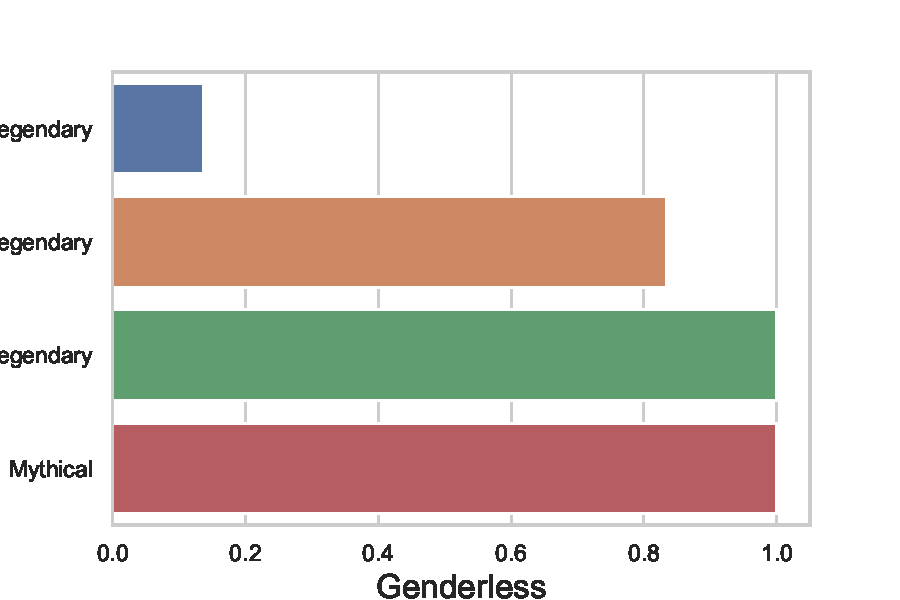
\includegraphics[width=\columnwidth]{../../figures/bar_genderless.pdf}
	\centering
	\caption{Barplot of the \textit{Genderless} distribution among different Pokémon labels, sorted by the relative frequency of Pokémon having no gender.}
	\label{fig:genderless}
\end{figure}
As shown by figure \ref{fig:genderless} all \textit{Legendary} and \textit{Mythical} Pokémon are genderless, whereas only $80\%$ of \textit{Sub-Legendary} Pokémon show the same property. The frequency of \textit{Non-Legendary} Pokémon, however, is nearly not noticeable. Roughly $10\%$ of these Pokémon have no gender. This leads us to another hypothesis:
\begin{enumerate}
	\setcounter{enumi}{4}
	\item \textit{Legendary}, \textit{Mythical} and \textit{Sub-Legendary} Pokémon show no gender at all.
\end{enumerate}
Furthermore, we can use this information to implement a simple classifier. For this we summarize specific class labels and aggregate them to a generic class label, simply called \textit{Legendary}. Each Pokémon that is either \textit{Legendary}, \textit{Sub-Legendary} or \textit{Mythical} will be assigned to the class $1$. \textit{Non-Legendary} Pokémon will be assigned to class $0$. Then, we construct a classifier as follows
\begin{equation}
	predict(x_{genderless}) = 
	\begin{cases}
		1 \quad \mathtt{if} \ x_{genderless} = 1 \\
		0 \quad \mathtt{else}
	\end{cases}
\end{equation}
where $x_{genderless}$ is $1$ for a given Pokémon if it has indeed no gender. Using this classifier on all Pokémon reaches an \textit{accuracy} score of $0.869$. This is one minus the proportion of genderless Pokémon among the \textit{Non-Legendary} Pokémon falsely predicted as $1$. This classifier, however, does worse than the simple baseline model, that predicts ever Pokémon as \textit{Non-Legendary} (see section \ref{subsec:scraping})

\subsection{Legendary Typing}
In this section, we highlight the importance of a Pokémon's first and second \textit{Type} regarding the given classification task. Based on our data, a Pokémon can have one of $18$ Types\footnote{For a list of available Types see: https://bulbapedia.bulbagarden.net/wiki/Type.}. More than half the Pokémon in a given category also have a second \textit{Type}.
\begin{table}[b]
	\centering
	\caption{Shows the distribution of None Types, that is Pokémon with no second Type among the different classes of Pokémon in percentages.}
	\label{tab:types}
	\begin{tabular}{lr} \hline
		\textbf{Class} & \textbf{None Type-Frequency} \\ \hline
		Legendary      & 0.217                        \\
		Sub-Legendary  & 0.409                        \\
		Mythical       & 0.483                        \\
		Non-Legendary  & 0.405                        \\ \hline
	\end{tabular}
\end{table}
\begin{table*}[t!]
	\centering
	\caption{Contingency table of Label and Type1 (Type2) among all Pokémon shown as relative frequencies of all Pokémon sharing the same Label. Highlighted are the most frequent types. Only columns are shown, where the relative frequency in one cell is equal or greater than $0.05$, thus only showing important Types.}
	\label{tab:type1}
	\begin{tabular}{lrrrrrrrrrrrr}
		\toprule
		Type1 &   Bug &  Dark &  Dragon &  Electric &  Fairy &  Fire &  Grass &  Normal &  Psychic &  Rock &  Steel &  Water \\
		Label         &       &       &         &           &        &       &        &         &          &       &        &        \\
		\midrule
		Legendary     &  0.00 &  0.04 &    \textbf{0.22} &      0.00 &   0.09 &  0.04 &   0.00 &    0.00 &    \textbf{ 0.30} &  0.00 &   0.04 &   0.09 \\
		Mythical      &  0.05 &  0.09 &    0.00 &      0.05 &   0.00 &  0.05 &   0.05 &    0.09 &     \textbf{0.23} &  0.05 &  \textbf{ 0.18} &  0.14 \\
		Non Legendary &  0.09 &  0.04 &    0.03 &      0.05 &   0.02 &  0.06 &   0.10 &    \textbf{0.13} &     0.05 &  0.06 &   0.03 &  \textbf{ 0.14} \\
		Sub Legendary &  0.05 &  0.02 &    0.05 &      \textbf{0.12} &   0.00 &  0.10 &   0.07 &    0.07 &    \textbf{ 0.12} &  0.10 &   0.07 &   0.05 \\
		\bottomrule
	\end{tabular}
	\\ \ \\ \ \\
	\begin{tabular}{lrrrrrrrrrr}
		\toprule
		Type2 &  Dragon &  Fairy &  Fighting &  Fire &  Flying &  Ghost &  Grass &  None &  Psychic &  Steel \\
		Label         &         &        &           &       &         &        &        &       &          &        \\
		\midrule
		Legendary     &    \textbf{0.17} &   0.00 &      0.04 &  0.09 &    \textbf{0.17} &   0.04 &   0.00 & \textbf{ 0.22} &     0.00 &   0.13 \\
		Mythical      &    0.00 &   0.09 &      0.05 &  0.05 &    0.05 &   0.09 &   0.09 &  \textbf{0.41} &     0.09 &   0.05 \\
		Non Legendary &    0.03 &   0.04 &      0.02 &  0.02 &    \textbf{0.11} &   0.02 &   0.02 &  \textbf{0.48} &     0.04 &   0.03 \\
		Sub Legendary &    0.05 &   0.10 &      0.12 &  0.00 &    \textbf{0.14} &   0.02 &   0.00 &  \textbf{0.40} &     0.05 &   0.07 \\
		\bottomrule
	\end{tabular}
\end{table*}
The exact distribution is shown in table \ref{tab:types}. Only $21.7\%$ of \textit{Legendary} Pokémon have no second \textit{Type}. $78.3\%$, however, have a second \textit{Type}. This allows for interesting Type-combinations among all Pokémon, of which some are more likely as others. Our research shows that the combination of (Grass, Poison), for example, is much more likely than (Grass, Rock). The most common type combination is (Flying, Normal), where almost $35\%$ of \textit{Flying}-Pokémon are \textit{Normal} as well.\\
Though, this finding does not help for the given classification task. Instead, we focus on the Type distribution among different classes of Pokémon. For this we use contingency tables for the two categorical values (Class, Type), where a Type can further be divided into First and Second Type.\\
The results are shown in table \ref{tab:type1}. Here, a cell entry indicates the relative frequency of, for example, all \textit{Legendary} Pokémon having the Type \textit{Bug} as a first Type, second Type respectively. The table shows, that one third of \textit{Legendary} Pokémon has \textit{Psychic} as their first Type, followed by the \textit{Dragon}-Type. In comparison, only $5\%$ of \textit{Non-Legendary} Pokémon are \textit{Psychic} and $3\%$ are \textit{Dragon}. This indicates, that belonging to a specific first or second Type can be an important factor to predict a Pokémon's \textit{Legendary} status. This effect is most prominent with the \textit{Psychic} Type as it shows to be a frequent Type among all Pokémon but \textit{Non-Legendary} Pokémon.\\
Looking at the table we can also tell, that \textit{Legendary} Pokémon never have \textit{Psychic} as their second Type. This is not true for \textit{Dragon}, though. Among the different classes of Pokémon, roughly $40\%$ have no second Type at all. Again, \textit{Legendary} Pokémon seem to be an exception, where only $22\%$ do not have a second Type. This gives rise to the question, whether \textit{Legendary} Pokémon get unique Type combinations. This might be true. Using contingency tales, we create a single table, combining the three categorical variables \textit{Label, Type1} and \textit{Type2} and again look at the relative frequency. Almost all Type combinations among \textit{Legendary} Pokémon show a frequency of roughly $4.5\%$. Considering that only $22$ Pokémon are \textit{Legendary}, this makes us believe, that unique Type combinations are especially important for these Pokémon. Of course, with more Pokémon sharing the same Label, this leads to an increased probability, that two Pokémon share the same Type combination. With $18$ Types and the possibility of no second Type the number of unique Type combinations is
\begin{equation}
	typecomb  = \frac{19!}{(19-2)!\cdot 2!}
		= \frac{19 \cdot 18}{2} 
	 = 171
\end{equation}
For $806$ \textit{Non-Legendary} Pokémon and an uniform distribution of type combinations this would mean, that about $4.7$ \textit{Non-Legendary} Pokémon would share the same Type combination or $0.58\%$, which is almost six times larger than $\frac{1}{806}$ or $0.12\%$.\\
We conclude this exploration with one last hypothesis:
\begin{enumerate}
	\setcounter{enumi}{5}
	\item A Pokémon's Type is an important indicator to predict, whether it belongs to the \textit{Legendary} or \textit{Non-Legendary} class.
\end{enumerate}
\FloatBarrier
\section{Decision Trees}
\label{sec:decision}
In the last section, we gave an exploratory insight into the difference among Pokémon belonging to different classes. We now want to give a quick theoretical overview on \textit{Decision Trees}, the primary exploratory model, we use in for the given classification task.\\
Decision Trees are an effective and popular classification method initially developed by Leo Breiman et al. \cite{breiman84} in 1984. Bruce P., Bruce A. and Gedeck define a Decision Tree in \cite[p. 250]{bruce17} as a "set of 'if-then-else' rules that are easy to understand and implement". For them one of the main advantages of decision trees lies in the easy explain-ability. In addition, in contrast to linear and logistic regression a decision tree is able to discover hidden patterns corresponding to complex interactions between predictors and the target variable in the data. A decision tree thus mimics the human decision making progress. Looking at loan data, a node in a decision tree may look at the borrower score of a given sample. If that score reaches a certain threshold, one may agree to the loan. When it is below the threshold, the loan is declined. This simple process can be visualized as a tree, where nodes stand for a decision and leafs for a final sub-division of the data into (hopefully) pure subsets.\\
In \cite{aurelien19}, Aurélien defines the impurity (1 - purity) of node $i$ as
\begin{equation}
	G_i = 1 - \sum_{k = 1}^{n} {p_{i, k}}^2
\end{equation}
where $p_{i, k}$ is the ratio of class $k$ instances among all instances in the $i^{th}$ node and $n$ the number of all classes. This means, when one node exists only of one class $k = 1$, then
\begin{equation}
	p_{i, k} =\begin{cases}
		1 & \mathtt{if} \quad k = 1 \\
		0 & \mathtt{else}
	\end{cases}
\end{equation}
The impurity this equals $0$, which is the best score. To achieve this, the decision tree algorithm will use the threshold for each predictor to reduce the impurity score as much as possible. Once the algorithm cannot improve the impurity significantly any more, the node becomes a leaf node. A decision tree with an impurity score of $0$ in each node would be a perfect decision tree.\\
Unfortunately, decision trees are prone to overfitting\footnote{See \cite[pp. 184]{aurelien19} for a more detailed explanation.}. A decision tree will adapt itself to the training data and thus perform worse on unseen or new data. One way to prevent this is using random forests instead \cite{liaw02}. Because random forest combine hundreds of randomized decision models in a bagging (Bootstrap Aggregation) approach, they loose some of the exploratory advantages of simpler decision trees. Instead we use \textit{Hyperparameter Regularization}.\\
Decision trees come with a lot of hyperparameters to prevent an overfit. To discriminate between \textit{Generic Legendary} and \textit{Non-Legendary} Pokémon we finetune the following hyperparameters with a $3$-fold cross validation, using a gridsearch in sklearn:
\begin{itemize}
	\item Maximum Depth
	\item Maximum number of Features
	\item Maximum number of Leaf-Nodes
	\item Minimum Samples a Leaf must contain
\end{itemize}
The decision tree model is evaluated for 6300 candidates and fitted 18900 times. We keep the model with the best accuracy score. One might also consider the F1-measure, as it prevents the model from ignoring infrequent classes. We did not encounter this problem, though.

\section{Results}

\section{Summary}

\begin{thebibliography}{00}
\bibitem{aalst16} Van Der Aalst, Wil: {\em "Data science in action."} Process mining. Springer, Berlin, Heidelberg, 2016. pp. 3-23.
\bibitem{fayyad96}Fayyad, Usama M., Gregory Piatetsky-Shapiro, und Padhraic Smyth: {\em "Knowledge Discovery and Data Mining: Towards a Unifying Framework."} KDD. Vol. 96. 1996.
\bibitem{breiman84}Breiman, Leo, et al.: {\em "Classification and regression trees"}. CRC press, 1984.
\bibitem{bruce17}Bruce, Peter, Andrew Bruce, and Peter Gedeck: "{\em Practical Statistics for Data Scientists: 50+ Essential Concepts Using R and Python}". O'Reilly Media, 2020.
\bibitem{aurelien19}Géron, Aurélien: {"\em Hands-on machine learning with Scikit-Learn, Keras, and TensorFlow: Concepts, tools, and techniques to build intelligent systems"}. O'Reilly Media, 2019.
\bibitem{liaw02}Liaw, Andy, and Matthew Wiener: {\em "Classification and regression by randomForest."} R news 2.3 (2002): 18-22.
\end{thebibliography}

\end{document}
